\section{Titles} \label{sec:titles}
A \src{DockTitle} is a \src{Component} that may show an icon, a text, some \src{DockAction}s or other information about a \src{Dockable}. Users often grab a \src{DockTitle} when they want to start a drag \& drop operation.

\begin{figure}[h]
\centering
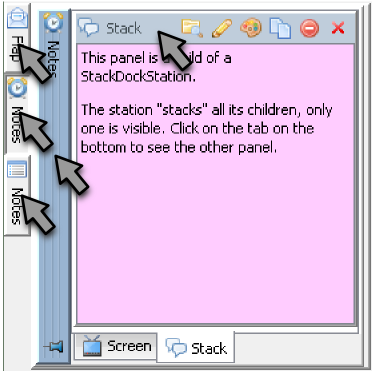
\includegraphics[scale=0.5]{titles/titles}
\caption{Some \src{DockTitles}.}
\label{fig:titles}
\end{figure}

\subsection{Lifecycle}
Any client that wants to show a \src{DockTitle} needs to specify what \textit{kind} of title it shows and needs to \textit{request} a title.

The \textit{kind} of a title is specified by a \src{DockTitleVersion}. New \linebreak \src{DockTitleVersion}s are obtained through the \src{DockTitleManager} (there is one per \src{DockController}). Creating a new \src{DockTitleVersion} requires the calling client to provide a default \src{DockTitleFactory}.

The \textit{request} for a title is handled by a \src{DockTitleRequest}. Once a \linebreak \src{DockTitleRequest} is created its method \src{request} can be called to execute the request. Clients should call \src{install} before using the request and \src{uninstall} once the request is no longer in use. This way the \src{DockTitleRequest} will automatically be executed again if the underlying \src{DockTitleFactory} is exchanged.

Once a \src{DockTitle} is acquired it must be connected with its \src{Dockable}. Clients must call the method \src{bind( DockTitle )} of \src{Dockable}, this tells the \src{Dockable} that is has a new title. If the client no longer shows the title it must call \src{unbind( DockTitle )}.

\warningbox{Do not call the method \src{bind} or \src{unbind} of \src{DockTitle}, these methods are called automatically by the \src{DockController}.}

\infobox{\src{Dockable}s provide some information about their titles:
\begin{itemize}
	\item The method \src{listBoundTitles} returns an list of all \src{DockTitle}s which are currently in use for the \src{Dockable}.
	\item A \src{DockableListener} has several methods that will be invoked if titles get added, removed, updated or exchanged.
\end{itemize}}

\subsection{Custom titles}
\subsubsection{Implementing a new title}
It is possible to replace all the titles in the framework. While the interface \src{DockTitle} is rather open, a title is responsible to collect all the information it wants to show by itself.

Most titles will have a constructor that has a \src{Dockable} as argument. They will add a \src{DockableListener} to their \src{Dockable} once \src{bind} is called and remove the listener once \src{unbind} is called.

There is only one connection between a module that shows a title and the title itself: the method \src{changed}. Modules use this method to send \linebreak \src{DockTitleEvent}s to the title.

\designbox{A module does not need to know what title it shows. It just delivers the \src{DockTitleEvent} to the title. The module can use a subclass of \src{DockTitleEvent} to transfer more information than \src{DockTitleEvent} alone could carry. This design allows to use any implementation of \src{DockTitle} at any place while some titles still can use additional information from their environment. An example is the \src{EclipseDockTitleEvent} which is used by tabs. This event also tells the titles at which location they are and whether their tab is focused or not.}

There are some classes that can help implementing a custom title:
\begin{itemize}
	\item \src{AbstractDockTitle} provides standard implementations for most of the features a title requires. Subclasses only need to override the method \linebreak \src{paintBackground} to have their custom painting code used.
	\item \src{BasicDockTitle} paints some gradients as background. Clients can change the color of these gradients. This title is also a good reference of how things can be done.
	\item \src{ButtonPanel} is a \src{Component} able to display a set of \src{DockAction}s. \linebreak \src{ButtonPanel} is able to show a popup-menu if there is not enough space for all actions.
\end{itemize}

\classbox{In order to use the popup menu of \src{ButtonPanel} some special code has to be written. First: the argument \src{menu} of the constructor of \src{ButtonPanel} has to be set to \src{true}. Second: the method \src{getPreferredSize} of \src{ButtonPanel} cannot be used, any standard \src{LayoutManager} will fail. Instead the method \src{doLayout} of the \src{Container} which shows the panel can be overriden. In this \src{doLayout} method the container should call \src{getPreferredSizes} to obtain a list of possible sizes of the panel. The $n$'th dimension in this array tells how big the \src{ButtonPanel} would be if it would show $n$ actions. The container should choose the biggest possible $n$ and call \src{setVisibleActions}.}

\codebox{An example showing a custom title is ``DockTitle: Custom title''.}

\subsubsection{Apply the title}
There are several ways to introduce a custom title into the framework.

To override or implement \src{requestDockTitle} of \src{Dockable} is the simplest way. The method just creates a new instance of the custom title when called.

Overriding or implementing \src{requestChildDockTitle} of \src{DockStation} allows to exchange the title of all children.

The \src{DockTheme} can be used as well. Either override the method \linebreak \src{getTitleFactory} or call \src{setTitleFactory} when using a \src{BasicTheme}. With a few exceptions all the modules use the factory of the theme, hence replacing this factory will have a big effect.

Or use the \src{DockTitleManager} to make some better tuned settings. The \linebreak \src{DockTitleManager} can be accessed by calling \src{getDockTitleManager} of \linebreak \src{DockController}. Search the unique string identifier of the module that uses a title and call \src{getVersion} to access the associated \src{DockTitleVersion}. Then with the help of \src{setFactory} a new factory can be introduced. In code this could look like this:
\begin{lstlisting}
DockController controller = ...

DockTitleManager manager = controller.getDockTitleManager();
DockTitleVersion version =
  manager.getVersion( SplitDockStation.TITLE_ID, null );
version.setFactory( new CustomDockTitleFactory(), Priority.CLIENT );
\end{lstlisting}
